% performance

This chapter outlines the algorithms that reconstruct muons and evaluate the missing transverse energy. Furthermore, it describes the data-driven corrections that were applied to muons in Monte-Carlo to correct for defects that are not modeled in the simulation. These corrections are derived from \Zmm\ events, which serve as a standard candle in the tag-and-probe procedure.

\section{Muon Reconstruction}
\label{sec:event:muonperf}

\subsection{Trigger}
\label{sec:event:trig}
In order to select events with muons, ATLAS deploys several muon triggers that differ in the $p_T$ threshold, muon multiplicity in the final state, and underlying implementation. Muon candidates are first defined in the hardware-based Level-1 (L1) trigger, where coincidental hits within narrow Regions of Interest (ROI) are detected in RPC and TGC chambers (see Sec.~\ref{chap:det:id}). The L2 trigger refines these muon candidates by adding fine-grained information from MDT and CSC chambers, as well as the hits from the Inner Detector, that are contained within the ROI's. These refinements allow muons from cosmic rays and in-flight meson decays to be rejected. Finally, the Event Filter (EF) trigger has access to the full event data and performs nearly offline-quality reconstruction.

This analysis uses the lowest-$p_T$ unprescaled single-muon triggers. An unprescaled trigger is a trigger with a sufficiently high $p_T$ threshold (and therefore, low firing rate) that it is possible to save every event candidate that fires the trigger. For 2011 data, EF\_mu18 and EF\_mu18\_MG triggers were considered for data taking periods D-I, while EF\_mu18\_medium and EF\_mu18\_MG\_medium were considered for periods J-M. EF\_mu18 and EF\_mu18\_MG trigger chains are seeded by L1\_MU10 ROI's, which require coincidence in two muon spectrometer stations in detecting a $p_T>10$ GeV muon. The ``medium'' chains, owing to increased instantaneous luminosity, are seeded by L1\_MU11, which requires coincidence in three stations for $p_T>11$ GeV muons. Other than the L1 seed, the default and ``medium'' chains are exactly the same at the L2 and EF. ``MG'' stands for MuGirl - one of two muon reconstructions algorithms in ATLAS; triggers without ``MG'' in their name utilize the alternative Muid algorithm. Studies summarized in Appendix~\ref{appendix:ac} motivate the choice of the Muid version of the triggers in the nominal analysis.

All of EF\_mu18 triggers are designed to efficiently detect muons with $p_T >$ 18 GeV, leaving a $2$ GeV buffer zone before the lowest muon $p_T$ cut used in the analysis ($20$ GeV).

%% Fig.~\ref{fig:perf:plato} shows a typical trigger turn-on curve 

%% \begin{figure}[phtb]
%%   \begin{center}
%%     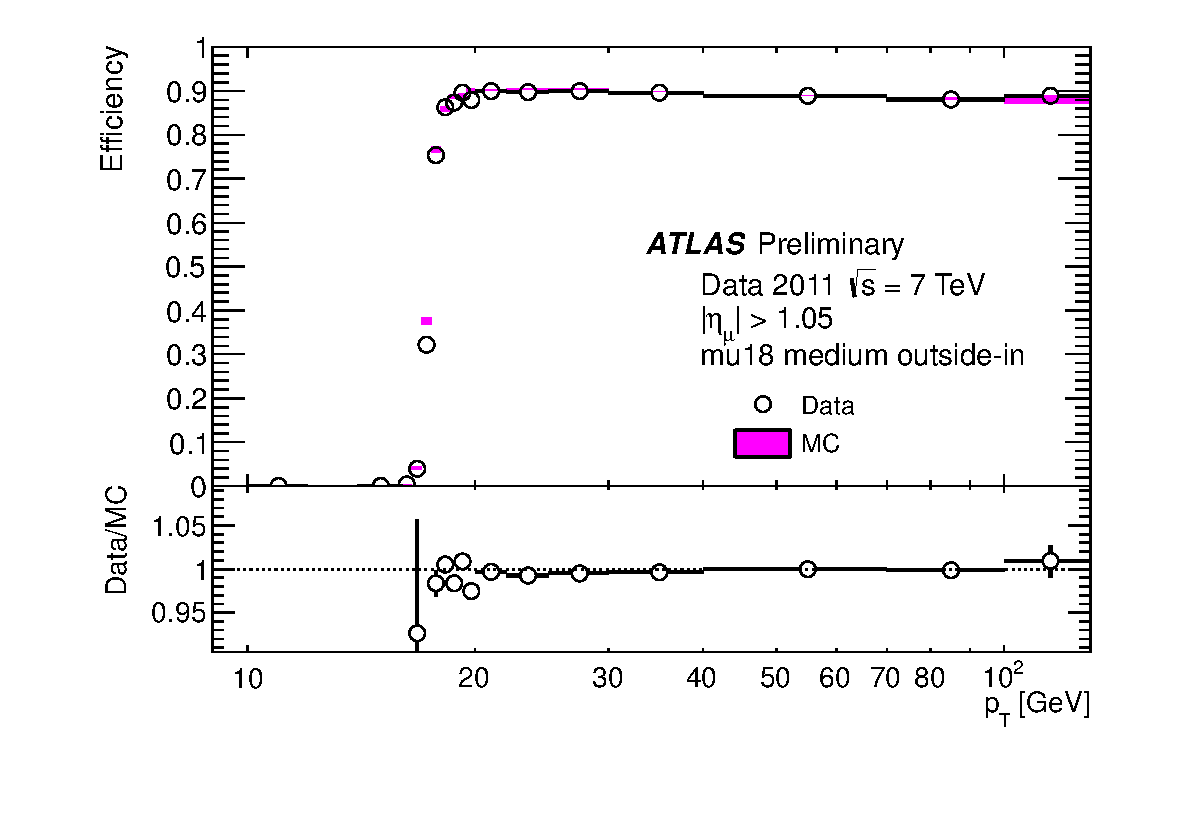
\includegraphics[width=0.70\textwidth]{perf/fig/mu18_turnon}
%%     \caption{ Trigger efficiency of mu18 triggers as a function of muon $p_T$. The trigger reaches its plateau before $p_T = 20~GeV$. }
%%     \label{fig:perf:plato}
%%   \end{center}
%% \end{figure}

\subsection{Muon Types}
Muons are reconstructed as tracks in the Inner Detector (Chap.~\ref{chap:det:id}) and ``Standalone'' muon candidates in the Muon Spectrometer (Chap.~\ref{chap:det:ms}). For high-precision analyses, such as the \Wmn\ cross-section measurement, the two measurements are combined to achieve the highest-quality of muon reconstruction and the best fake-muon rejection.

\paragraph{Inner Detector Tracks}
A typical inner detector track is reconstructed from 3 pixel hits, 8 SCT hits, and 30 TRT hits. The default reconstruction strategy is the ``inside-out'' strategy, which consists of the following steps~\cite{ATLAS-CONF-2012-042}:
\begin{itemize}
\item Three-dimensional spacepoints are formed from pixel and SCT hits.
\item Using pattern recognition, track seeds made of at least three spacepoints are formed.
\item A statistical algorithm called Kalman filter iteratively adds additional hits to the tracks while working outwards.
\item Track candidates are assigned a score based on the number of hits and holes. Low-quality and duplicate candidates are removed.
\item Surviving candidates are extrapolated into TRT. Tracks are re-fitted including TRT hits in the extrapolation region.
\item If the addition of TRT hits results in a lower track score, or if the extrapolation region is not instrumented with TRT modules, the original pixel+SCT track is retained.
\end{itemize}

\paragraph{Standalone Muons}
Standalone muons are constructed by recognizing consistent straight segments within at least two muon chambers that point to the center of the ATLAS detector. Two alternative algorithms are available: Muonboy and MOORE. Muonboy combines track segments through an iterative fitting procedure working outside-in, while MOORE is based on the Hough transform~\cite{leroy2010astroparticle}. Both algorithms extrapolate reconstructed muons to the Inner Detector, with Muonboy parametrizing calorimeter losses as a function of $\eta$ and $p_T$. MOORE supplements the parametrization with actual calorimeter measurements.

\paragraph{Combined Muons}
Standalone muons extrapolated to the Inner Detector are matched to ID tracks through a statistical combination of track parameters and covariances. Those candidates that pass the combination $\chi^2$ cuts are saved in the list of combined muons. Typically, the ID measurement dominates for muons with $p_T<40$ GeV, while more energetic muons are better constrained by the spectrometer.

As in the case of standalone muons, two algorithms exist for muon combination~\cite{muon_tdr}. The STACO algorithm uses MuonBoy candidates and obtains the helix parameters of a combined muon through a statistical combination with the ID track candidate, using the full correlation matrix. The MuId algorithm relies on MOORE standalone candidates and performs a full re-fit of the track including the inner detector hits.

The overall performance of the two algorithms is comparable, and both remain in use. This analysis relies on the STACO reconstruction chain and utilizes isolated STACO muons with additional track quality criteria to reconstruct \Wboson\ bosons (see Sec.~\ref{sec:event:fullsel}).

\section{Muon Corrections}
\label{sec:perf:muoncorr}

Simulating the passage of muons through the ATLAS detector is a complex task. Although test beam studies, cosmic ray calibrations, and studies of earlier collisions have produced an excellent detector model, the Monte-Carlo still suffers from a number of subleading effects, such as unaccounted inhomogeneities in the magnetic field, incorrect material distributions, subtle misalignments, or improperly modeled detector response. For a precision analysis, such as this one, these defects can doom the entire measurement.

Thankfully, nature provides a standard candle - the Z boson - that can be exploited to derive data-driven corrections that bring the efficiency of various cuts in data and Monte-Carlo into agreement. The procedure is commonly known as tag-and-probe, and relies on the correlation between the two muons in \Zmm\ decays. One muon is ``tagged'' with tight requirements, while the second one, called the ``probe'', is initially selected with all cuts minus the one that's under study - such as the requirement that the probe fired a trigger. Z selection is then applied to strongly correlate the two muons. This includes a tight cut on the invariant mass of the muon pair, as well as the requirement that the muons carry opposite charges. This ensures that even the loosely selected probes represent actual muons, as opposed to other objects mis-identified as muons. As the final step, the cut under study (e.g., trigger match) is applied to the probe. Distributions of kinematic variables ($\eta$, $p_T$, etc) of the probe before and after the final cut serve as the denominator and numerator of the efficiency ratio for that cut.

The procedure is separately repeated for data and uncorrected Monte-Carlo. The ratio of their respective efficiencies is a multiplicative scale factor. This scale factor is computed on a per-muon basis and applied to the Monte-Carlo event weight in the nominal analysis.

\subsection{Reconstruction Efficiency}
Reconstruction efficiency scale factors are derived from a standard tag-and-probe procedure, where the probe is either an Inner Detector (ID) track or a so-called CaloTag muon (an ID track with muon-like depositions in the calorimeter). These scale factors correct the combined efficiency of finding a muon candidate in the spectrometer and successfully matching it to the ID track.

Reconstruction scale factors are binned in ($q,\eta,\phi$). $\eta$ binning is chosen to match cross-section binning in the single and double-differential measurements. The scale factors generally stay within 1-2\% of 1, except for narrow $\eta$ regions at the interface between the Barrel and the Endcap, as illustrated in Fig.~\ref{fig:perf:recosf_sf}.

Systematic uncertainty is driven by two sources: choice of the probe, shown in Fig.~\ref{fig:perf:recosf_caloid}, and missing $p_T$-dependence (typically 0.1-0.2\%).

\begin{figure}[phtb]
  \begin{center}
  \includegraphics[width=1.0\textwidth]{MuonPerformance/figures/NewRecoSF/SF_etaPhi_negq}
 \caption{ Reconstruction scale factors for combined STACO muons, which are derived from Z tag-and-probe using ID tracks as probes.}
 \label{fig:perf:recosf_sf}
 \end{center}
\end{figure}

\begin{figure}[phtb]
  \begin{center}
 \includegraphics[width=1.0\textwidth]{MuonPerformance/figures/NewRecoSF/CaloDeviation_etaPhi_negq}
 \caption{ The difference in reconstruction scale factors when using CaloTag vs ID track probes, which contributes to the systematic uncertainty. }
 \label{fig:perf:recosf_caloid}
 \end{center}
\end{figure}

%% \begin{figure}[phtb]
%%   \begin{center}
%%         \subfigure[Reco. SF (nominal)]{%
%%           \includegraphics[width=0.85\textwidth]{MuonPerformance/figures/NewRecoSF/SF_etaPhi_negq}
%%         }
%%         \subfigure[ID track vs CaloTag as probe]{%
%%           \includegraphics[width=0.85\textwidth]{MuonPerformance/figures/NewRecoSF/CaloDeviation_etaPhi_negq}
%%         }
%%  \caption{ Top: reconstruction scale factors for combined STACO muons derived from Z tag-and-probe using ID tracks as probes. Bottom: difference in reconstruction scale factors when using CaloTag vs ID track probes, which contributes to the systematic uncertainty.}
%%  \label{fig:perf:recosf_sum}
%%  \end{center}
%% \end{figure}

%% \begin{figure}[phtb]
%%   \begin{center}
%%         \subfigure[Reco. SF: $\mu^-$]{%
%%           \includegraphics[width=0.44\textwidth]{MuonPerformance/figures/NewRecoSF/SF_etaPhi_negq}
%%         } 
%%         \subfigure[Reco. SF: $\mu^+$]{%
%%           \includegraphics[width=0.44\textwidth]{MuonPerformance/figures/NewRecoSF/SF_etaPhi_posq}
%%         }
%%  \caption{ Reconstruction scale factors for combined STACO muons. These scale factors were derived from Z tag-and-probe using ID tracks as probes.}
%%  \label{fig:perf:recosf}
%%  \end{center}
%% \end{figure}

%% \begin{figure}[phtb]
%%   \begin{center}
%%         \subfigure[ $\mu^-$]{%
%%           \includegraphics[width=0.44\textwidth]{MuonPerformance/figures/NewRecoSF/CaloDeviation_etaPhi_negq}
%%         } 
%%         \subfigure[ $\mu^+$]{%
%%           \includegraphics[width=0.44\textwidth]{MuonPerformance/figures/NewRecoSF/CaloDeviation_etaPhi_posq}
%%         }
%%  \caption{ Difference in reconstruction scale factors when using CaloTag vs ID track probes. This difference contributes to the systematic uncertainty.}
%%  \label{fig:perf:recosf_caloid}
%%  \end{center}
%% \end{figure}

\subsection{Isolation Efficiency}

The definition and motivation behind the muon isolation cut is described in Sec.~\ref{subsec:MuonIsolation}.

Isolation scale factors are derived from Z tag-and-probe events and correct the efficiency of the isolation cut in Monte-Carlo. Isolation scale factors are binned in $p_T$ only, since they were found to be flat in other variables (Fig.~\ref{fig:perf:isosf}). Systematic uncertainty is derived by varying Z tag-and-probe selection cuts by $\pm 10\%$ and adding significant variations in quadrature. The typical uncertainty is 0.1\%.

\begin{figure}[phtb]
  \begin{center}
        \subfigure[Isolation SF: $\eta$]{%
          \includegraphics[width=0.44\textwidth]{MuonPerformance/figures/eff_cb_isoid40rel01_mu_probe_eta}
        } 
        \subfigure[Isolation SF: $p_T$]{%
          \includegraphics[width=0.44\textwidth]{MuonPerformance/figures/eff_cb_isoid40rel01_mu_probe_pt}
        }
 \caption{ Isolation scale factors for the $\frac{p_T^\mathrm{cone40}}{p_T^{\mu}} < 0.1$ cut used in the analysis.}
 \label{fig:perf:isosf}
 \end{center}
\end{figure}

\subsection{Trigger Efficiency}
Trigger scale factors are derived from Z tag-and-probe events, where the probe is required to explicitly match to one of Event Filter trigger objects in a $\Delta R < 0.1$ cone.

Trigger scale factors are binned in ($\eta,p_T,q$), where both $\eta$ and $p_T$ match the binning used in the single and double-differential measurements. The scale factors are computed separately for several data period sub-ranges in order to account for different runtime trigger configurations throughout 2011. Trigger scale factors generally stay within 5\% of 1, but in some pathological cases (Fig.~\ref{fig:perf:trigsf}) may reach 30\%.

Systematic uncertainty is driven by the the lack of $\phi$ parametrization, which could not be added due to insufficient tag-and-probe statistics in the period sub-ranges. This systematic is typically 0.1-0.3\%.

\begin{figure}[phtb]
  \begin{center}
        \subfigure[Trigger SF: $\mu^-$, periods G-I]{%
          \includegraphics[width=0.85\textwidth]{MuonPerformance/figures/scaleFactors/mu18_neg_SF_eta_pt}
        }
        \subfigure[Reco SF: $\mu^+$, periods L3-L4]{%
          \includegraphics[width=0.85\textwidth]{MuonPerformance/figures/scaleFactors/rpc_pos_SF_eta_pt}
        }
 \caption{ Trigger scale factors for mu18 Muid triggers, derived from Z tag-and-probe events. The plot on the right shows the effect of a known RPC misconfiguration in periods L3 and L4, which resulted in large trigger inefficiency in data. }
 \label{fig:perf:trigsf}
 \end{center}
\end{figure}

\subsection{Momentum Resolution and Scale}
\label{perf:muon:scale}
In addition to scale factors to correct Monte-Carlo efficiency of various cuts, a separate correction is needed for the muon momentum.

Muon momentum resolution corrections are derived from \Zmm\ events and curvature differences between ID and spectrometer muons, using the fitting procedure described in~\cite{Cerutti:1322424}. The corrections are derived separately for ID and standalone muon and then propagated to combined muons.

In addition to these resolution terms, corrections are applied to the transverse momentum of the muons
in Monte-Carlo events to improve their agreement with the data. This is necessary to correct the bias
in muon momentum in 2011 Monte-Carlo due to an incorrect multiple scattering model (``Wentzel'') in the Geant4 simulation.
Additionally, these corrections take into account any remaining muon momentum mismodeling due to
detector and magnetic field effects that are not already covered by the resolution corrections.

First, the overall momentum scale (``K'') is set based on the location of the \Zmm\ peak in data and Monte-Carlo.
The uncertainty on the overall momentum scale is derived by varying the cuts used in the \Zmm\ selection, 
and by considering either a full analytic lineshape fit or an iterative Gaussian fit in the core of the invariant mass spectrum~\cite{Kapliy:1358186}.
Second, the component of muon momentum that's anti-correlated between charges (curvature ``C'') is corrected by balancing
positive and negative muons against each other in \Zmm\ events in data. The uncertainty on the curvature correction is
similarly derived by varying the cuts used in the \Zmm\ selection, and by employing two different methods to compute
the corrections (one based on a binned $\chi^{2}$ fit, and another based on unbinned Kolmogorov-Smirnov statistic).

The precise definition of these muon momentum correction parameters is shown below, where it is assumed that all momenta are given in GeV:
$$K \equiv \frac{M_{Z}^{data}}{M_{Z}^{MC}} \approx \frac{p_{T}^{measured}}{p_{T}^{corrected}}$$
$$\frac{1}{p_{T}^{corrected}} \equiv \frac{1}{p_{T}^{measured}} + (charge \cdot C)$$

The effect of muon momentum scale corrections on the reconstructed \Zmm\ peak in Monte-Carlo is illustrated in Fig.~\ref{fig:perf:mcpcorr}.

\begin{figure}[phtb]
  \begin{center}
        \subfigure[Before scale corrections]{%
          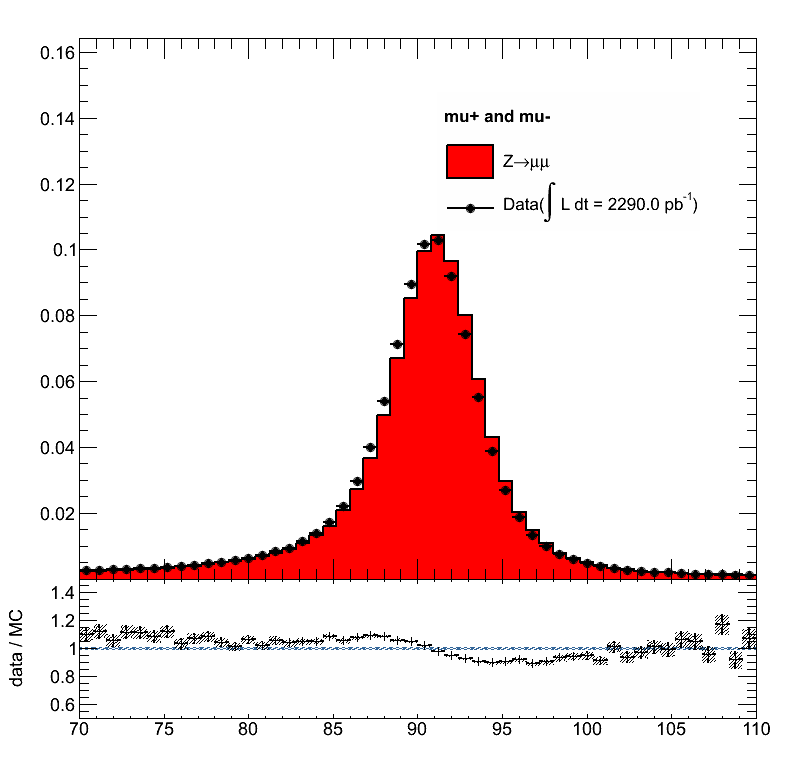
\includegraphics[width=0.44\textwidth]{perf/fig/KC_old}
        } 
        \subfigure[After scale corrections]{%
          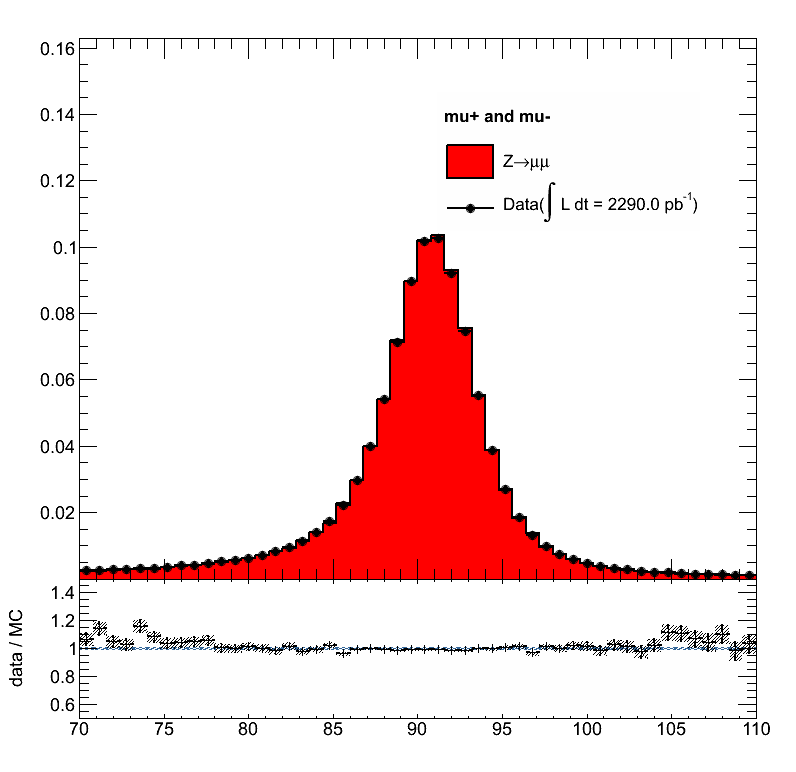
\includegraphics[width=0.44\textwidth]{perf/fig/KC_new}
        }
 \caption{ Effect of muon momentum scale corrections on the reconstructed \Zmm\ mass peak.}
 \label{fig:perf:mcpcorr}
 \end{center}
\end{figure}

\section{Missing Transverse Energy}
\label{perf:met:scale}
% https://cds.cern.ch/record/1548310/files/CERN-THESIS-2013-037.pdf
% https://indico.cern.ch/getFile.py/access?contribId=1&resId=0&materialId=slides&confId=161247

Missing transverse energy (\met) is used as a proxy for neutrino $p_T$ in \Wmn\ decays. Neutrinos interact with material so weakly that they always escape the detector, leaving an energy imbalance in the calorimeter. \met\ is defined as the transverse portion of this imbalance.

This analysis relies on the MET\_RefFinal algorithm to calculate \met~\cite{ATLAS-CONF-2012-101, Aad:2012re}. Calorimeter cells are first associated with the physics objects (muons, electrons, ...) and calibrated according to the object type, and then added vectorially. An additional adjustment is made for the muon momentum.

Because a calorimeter cell can be associated with multiple reconstructed objects, care must be taken to ensure that each cell contributes to \met\ calculation only once. This is accomplished by choosing the calibration for each cell in the following order of priority:
\begin{itemize}
\item MET\_RefEle - electrons
\item MET\_RefGamma - photons
\item MET\_RefTau - $\tau$ leptons that decayed hadronically
\item MET\_RefJet - jets with $p_T>20\ GeV$
\item MET\_RefMuon - energy deposited by muons in the calorimeter (usually a few GeV)
\item MET\_SoftJet - jets with $p_T<20\ GeV$
\item MET\_CellOutEflow - calorimeter cells not associated with any object
\end{itemize}

Additionally, a MET\_MuonBoy term, representing muon $p_T$, is added to the \met\ calculation because muons deposit only a small amount of their energy in the calorimeter

All analysis-level corrections to various event objects, such as corrections of the muon momentum or jet energy, are propagated to \met. The \MET\ uncertainty due to soft terms (cells that are not associated to any physics object) is evaluated by studying fake \MET\ in Z events and by comparing tracker and calorimeter measurements of electron momentum (E/p). The soft terms uncertainty is provided separately for \MET\ resolution and scale, and includes the effects of pileup on the calorimeters.

\subsection{Jet Reconstruction}
Although jets are not used explicitly in this analysis, they must be measured well to ensure a reliable estimation of missing transverse energy.

Jets are reconstructed from calorimeter topo-clusters (topologically connected groups of cells with energy deposition) using the anti-kT algorithm with cone size 0.4~\cite{Cacciari:2008gp}. They are subsequently calibrated using a four-step procedure illustrated in Fig.~\ref{fig:perf:jetcalib}. Further details are available in reference~\cite{ATLAS-CONF-2013-004}.

\begin{figure}[phtb]
  \begin{center}
    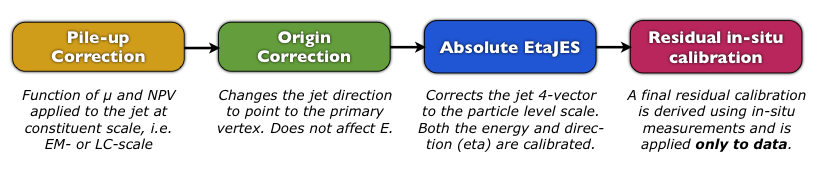
\includegraphics[width=0.99\textwidth]{perf/fig/calib}
 \caption{ An overview of the jet calibration scheme in ATLAS. A series of corrections are derived and applied to jet energy and direction.}
 \label{fig:perf:jetcalib}
 \end{center}
\end{figure}
